\documentclass{article}
\usepackage{graphicx}
\usepackage[utf8]{inputenc}
\usepackage{listings}
\usepackage{color}
\usepackage{xcolor}
\usepackage{textcomp}
\usepackage{amsmath}
\usepackage{mathabx}

\definecolor{solarized@base03}{HTML}{002B36}
\definecolor{solarized@base02}{HTML}{073642}
\definecolor{solarized@base01}{HTML}{586e75}
\definecolor{solarized@base00}{HTML}{657b83}
\definecolor{solarized@base0}{HTML}{839496}
\definecolor{solarized@base1}{HTML}{93a1a1}
\definecolor{solarized@base2}{HTML}{EEE8D5}
\definecolor{solarized@base3}{HTML}{FDF6E3}
\definecolor{solarized@yellow}{HTML}{B58900}
\definecolor{solarized@orange}{HTML}{CB4B16}
\definecolor{solarized@red}{HTML}{DC322F}
\definecolor{solarized@magenta}{HTML}{D33682}
\definecolor{solarized@violet}{HTML}{6C71C4}
\definecolor{solarized@blue}{HTML}{268BD2}
\definecolor{solarized@cyan}{HTML}{2AA198}
\definecolor{solarized@green}{HTML}{859900}

\lstset{
  language=Java,
  upquote=true,
  columns=fixed,
  tabsize=2,
  extendedchars=true,
  breaklines=true,
  frame=single,
  numbers=left,
  numbersep=5pt,
  rulesepcolor=\color{solarized@base03},
  numberstyle=\tiny\color{solarized@base01},
  basicstyle=\footnotesize\ttfamily,
  keywordstyle=\color{solarized@green},
  stringstyle=\color{solarized@cyan}\ttfamily,
  identifierstyle=\color{solarized@blue},
  commentstyle=\color{solarized@base01},
  emphstyle=\color{solarized@red}
}
\begin{document}

\title{Tarea Método de la Secante}
\author{Angel Caceres Licona}

\maketitle


\section{Termine las iteraciones y verifique sus resultados con la tabla 2}
Yo lo que hice fue programar el método y correrlo con los mismos datos.
Obtuve resultados idénticos:

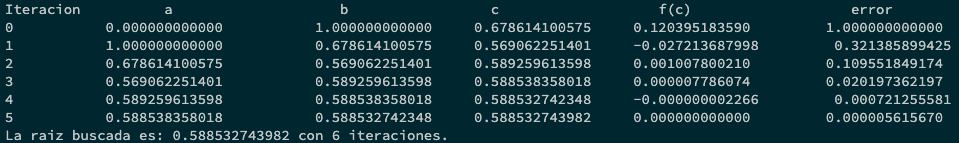
\includegraphics[scale=0.4]{resultadoSecante.png}

\section{Código del programa}

\begin{lstlisting}
    from math import *

    def fx(x):
        respuesta = -8*exp(1-x) + 7/x
        return respuesta
    
    
    def secante(a,b,tol):
        fa = fx(a)
        fb = fx(b)
        c = b - fb*((b-a)/(fb-fa))    
        i = 1
        error = abs(b-a)
        fc = fx(c)
        print "Iteracion          a                    b                 c                   f(c)                   error "
        for i in range (1000):
            c = b - (fb*(b-a)/(fb-fa))
            fc = fx(c)
            print "%.0f" %i, "          %.12f" %a,"          %.12f" %b,"    %.12f" %c, "    %.12f" %fc, "        %.12f" %error
            i = i+1
            if (fc==0.0 or abs(b-a) < tol):
                break
    
            a = b
            b = c
            fa = fx(a)
            fb = fx(b)
            
            error = abs(b-a)
    
        print "La raiz buscada es: %.12f" %c, "con " + str(i) + " iteraciones."
    
    secante(0.5,0.6,0.000000005)
\end{lstlisting}

\section{Considerar la función $f(x) = x^2-4\cos(x) , x \in {\rm I\!R}$...}
\subsection{Graficar $f(x)$ en el intervalo $1,2)$.}
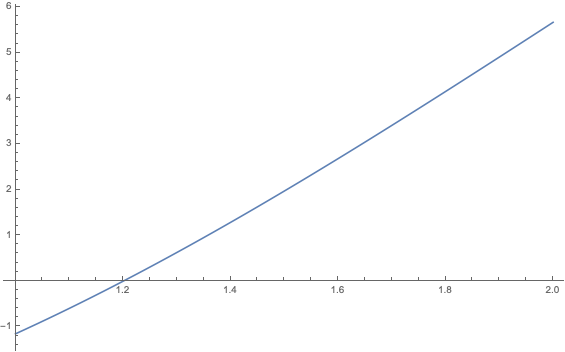
\includegraphics[scale=0.75]{grafica.png}

\subsection{Usar el método de la secante para localizar una aproximacion...}
Usando mi programa obtuve los siguientes resultados:

\begin{center}
    \begin{tabular}{||c c c c c c||} 
    \hline
    $n$ & $p_{n-1}$ & $p_{n}$  & $p_{n+1}$ & $|p_n - p_{n-1}|$ & $f(x_n)$\\ [0.5ex] 
    \hline\hline
    0 & 1 & 2 & 1.170120690182 & 1 & -0.190979794047 \\ 
    \hline
    1 & 2 & 1.170120690182 & 1.170120690182 & 1.197187270733 & 0.829879309818 \\
    \hline
    2 & 1.170120690182 & 1.197187270733 & 1.201577567782  & -0.190979794047 & 0.027066580551\\
    \hline
    3 & 1.197187270733 & 1.201577567782 & 1.201538251243 & -0.026654203791 & 0.004390297049\\
    \hline
    4 & 1.201577567782 & 1.201538251243 & 1.201538299340  & 0.000240853997 & 0.000039316539\\ [1ex]
    \hline

   \end{tabular}
\end{center}

\subsection{Aplicar el método de bisección con la misma tolerancia...}
Se requirieron 29 iteraciones para obtener un resultado similar, por lo que vemos que el método de bisección es mucho mas lento.
\begin{center}
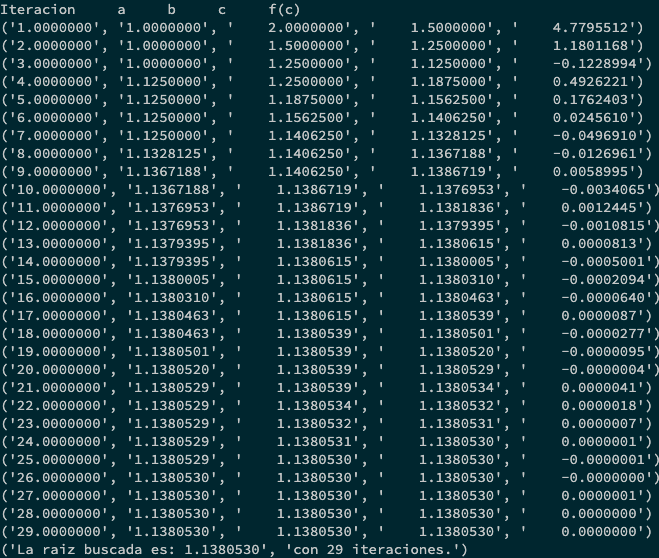
\includegraphics[scale=0.5]{salidaBiseccion.png}    
\end{center}
\section{Considere la función $f(x) = -8e^{1-x} + \frac{7}x{}$}
\subsection{Grafique en $(0,2)$ y verifique que tiene dos raíces.}
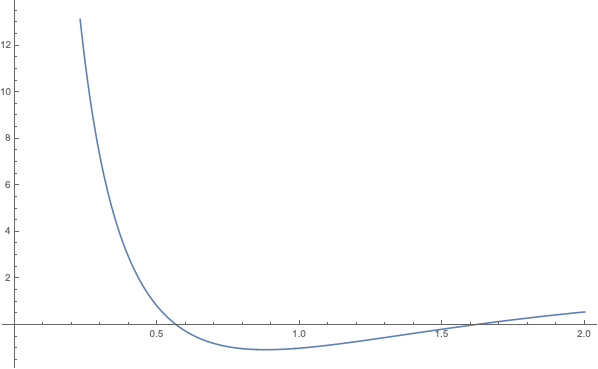
\includegraphics[scale=0.5]{grafica2.png}   
\subsection{Poner los resultados de cada raíz en una tabla}
Para la primer raíz tenemos: 

\begin{center}
    \begin{tabular}{||c c c c c c||} 
    \hline
    $n$ & $p_{n-1}$ & $p_{n}$  & $p_{n+1}$ & $|p_n - p_{n-1}|$ & $f(x_n)$\\ [0.5ex] 
    \hline\hline
    0 & 0.5 & 0.6 & 0.575149260929 & -0.064143321099 & 1 \\ 
    \hline
    1 & 0.6 & 0.575149260929  & 0.567327347390 & 0.007582973043 & -0.064143321099 \\
    \hline
    2 & 0.575149260929 & 0.567327347390 & 0.568154287638 & -0.000182851406 & 0.007821913540\\
    \hline
    3 & 0.567327347390 & 0.568154287638 & 0.568134816790 & -0.000000504095 & 0.000826940249\\
    \hline
    4 & 0.568154287638 & 0.568134816790 & 0.568134762964 & 0.000000000034 & 0.000019470848\\
    \hline 
    5 & 0.568134816790 & 0.568134762964 & 0.568134762967 & 0.000000000000 & 0.000000053827\\ [1ex]
    \hline

   \end{tabular}
\end{center}


Para la segunda raíz tenemos: 

\begin{center}
    \begin{tabular}{||c c c c c c||} 
    \hline
    $n$ & $p_{n-1}$ & $p_{n}$  & $p_{n+1}$ & $|p_n - p_{n-1}|$ & $f(x_n)$\\ [0.5ex] 
    \hline\hline
    0 & 1.55 & 1.62 & 1.609561727949 &  0.000297514517 & 0.07 \\ 
    \hline
    1 & 1.620000000000 & 1.609561727949  & 1.609380484711 & -0.000000960168 & 0.010438272051 \\
    \hline
    2 & 1.609561727949 & 1.609380484711 & 1.609381067755 & 0.000000000052 & 0.000181243238\\
    \hline
    3 & 1.609380484711 & 1.609381067755 & 1.609381067723 & 0.000000000000 & 0.000000583044\\ [1ex]
    \hline

   \end{tabular}
\end{center}

\subsection{Aplicar el método de bisección con la misma tolerancia...}
Se requirieron 26 iteraciones para obtener un resultado similar, para la 1er raiz:

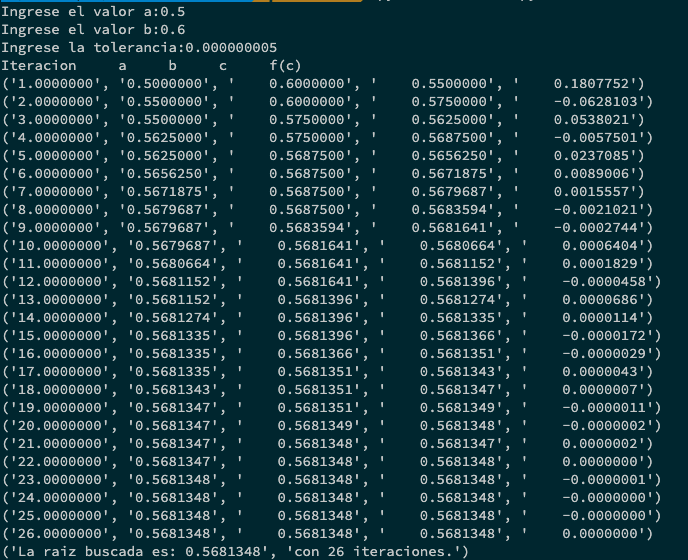
\includegraphics[scale=0.5]{salidaBiseccion1erRaiz.png} 

Se requirieron 25 iteraciones para obtener un resultado similar, para la 2a raiz:

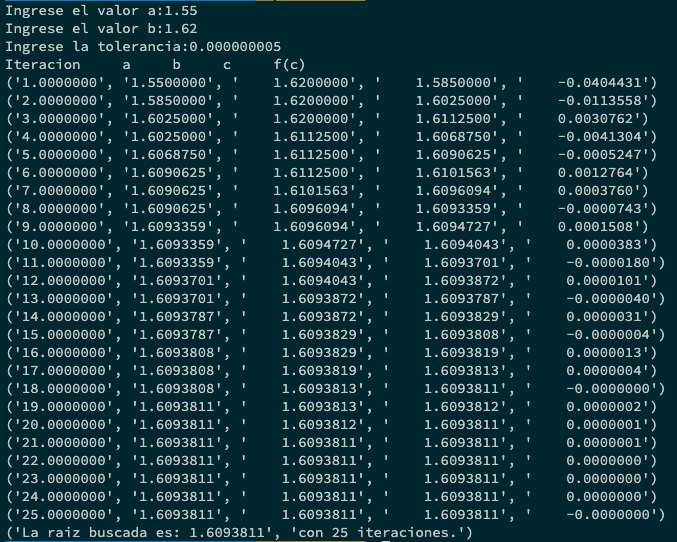
\includegraphics[scale=0.5]{salidaBiseccion2aRaiz.png} 


\end{document}